\begin{figure}[H]
    \begin{center}
        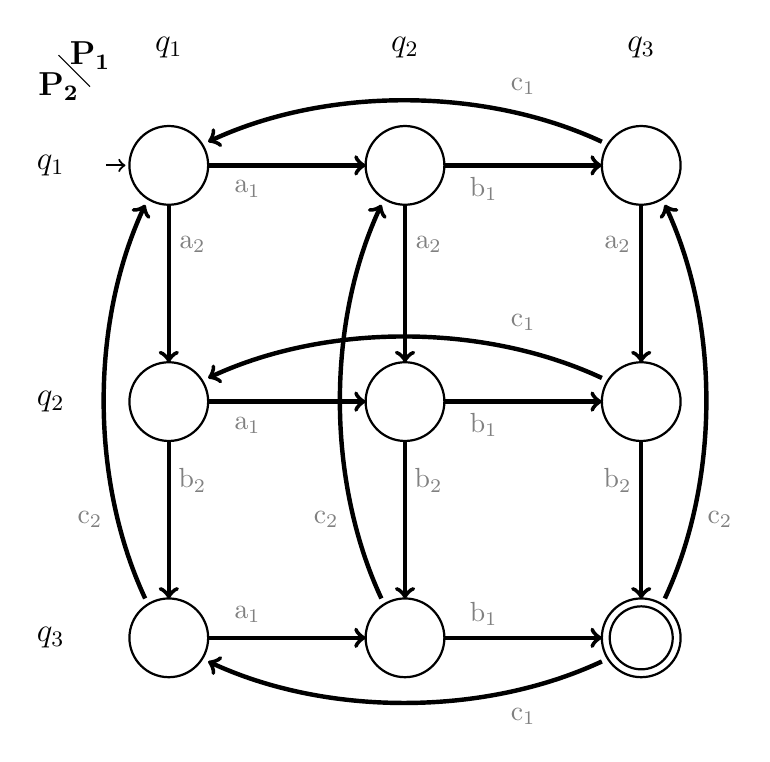
\begin{tikzpicture}
        %labels
        \draw(-1.0, 1.4) node [font = \large] {$\mathbf{P_1}$};
        \draw (-1.4, 1.4) -- (-1.0, 1.0);
        \draw(-1.4, 1.0) node [font = \large] {$\mathbf{P_2}$};
        
        \draw(0,1.5) node [font = \large] {$q_1$};
        \draw(3,1.5) node [font = \large] {$q_2$};
        \draw(6,1.5) node [font = \large] {$q_3$};
        
        \draw(-1.5,0)  node [font = \large] {$q_1$};
        \draw(-1.5,-3) node [font = \large] {$q_2$};
        \draw(-1.5,-6) node [font = \large] {$q_3$};
        
        %States
        \draw[thick, ->] (-0.8, 0) -- (-0.55, 0);
        \draw[color=black, thick](0,0) circle (0.5);
        \draw[color=black, thick](0,-3) circle (0.5);
        \draw[color=black, thick](0,-6) circle (0.5);
        \draw[color=black, thick](3,0) circle (0.5);
        \draw[color=black, thick](3,-3) circle (0.5);
        \draw[color=black, thick](3,-6) circle (0.5);
        \draw[color=black, thick](6,0) circle (0.5);
        \draw[color=black, thick](6,-3) circle (0.5);
        \draw[color=black, thick](6,-6) circle (0.5);
        \draw[color=black, thick](6,-6) circle (0.4);
        
        %Edges
            %horizontal 
            
        \draw[gray](4.5, 1) node {$\mathrm{c_1}$};
        \draw[color=black, ultra thick, <-] (0.5, 0.3) .. controls (2, 1) and (4, 1) .. (5.5, 0.3);
        
        \draw[gray](1, -0.3) node {$\mathrm{a_1}$};
        \draw[color=black, ultra thick, ->] (0.5, 0) -- (2.5, 0);
        
        \draw[gray](4, -0.3) node {$\mathrm{b_1}$};
        \draw[color=black, ultra thick, ->] (3.5, 0) -- (5.5, 0);
    
        
        \draw[gray](4.5, -2) node {$\mathrm{c_1}$};
        \draw[color=black, ultra thick, <-] (0.5, -2.7) .. controls (2, -2) and (4, -2) .. (5.5, -2.7);
        
        \draw[gray](1, -3.3) node {$\mathrm{a_1}$};
        \draw[color=black, ultra thick, ->] (0.5, -3) -- (2.5, -3);
        
        \draw[gray](4, -3.3) node {$\mathrm{b_1}$};
        \draw[color=black, ultra thick, ->] (3.5, -3) -- (5.5, -3);
        
        
        \draw[gray](4.5, -7) node {$\mathrm{c_1}$};
        \draw[color=black, ultra thick, <-] (0.5, -6.3) .. controls (2, -7) and (4, -7) .. (5.5, -6.3);
        
        \draw[gray](1, -5.7) node {$\mathrm{a_1}$};
        \draw[color=black, ultra thick, ->] (0.5, -6) -- (2.5, -6);
        
        \draw[gray](4, -5.7) node {$\mathrm{b_1}$};
        \draw[color=black, ultra thick, ->] (3.5, -6) -- (5.5, -6);
        
        
            %vertical
            
        \draw[gray](-1, -4.5) node {$\mathrm{c_2}$};
        \draw[color=black, ultra thick, <-] (-0.3, -0.5) .. controls (-1, -2) and (-1, -4) .. (-0.3, -5.5);
        
        \draw[gray](0.3, -1) node {$\mathrm{a_2}$};
        \draw[color=black, ultra thick, ->] (0, -0.5) -- (0, -2.5);
        
        \draw[gray](0.3, -4) node {$\mathrm{b_2}$};
        \draw[color=black, ultra thick, ->] (0, -3.5) -- (0, -5.5);
        
        
        \draw[gray](2, -4.5) node {$\mathrm{c_2}$};
        \draw[color=black, ultra thick, <-] (2.7, -0.5) .. controls (2, -2) and (2, -4) .. (2.7, -5.5);
        
        \draw[gray](3.3, -1) node {$\mathrm{a_2}$};
        \draw[color=black, ultra thick, ->] (3, -0.5) -- (3, -2.5);
        
        \draw[gray](3.3, -4) node {$\mathrm{b_2}$};
        \draw[color=black, ultra thick, ->] (3, -3.5) -- (3, -5.5);
        
        
        \draw[gray](7, -4.5) node {$\mathrm{c_2}$};
        \draw[color=black, ultra thick, <-] (6.3, -0.5) .. controls (7, -2) and (7, -4) .. (6.3, -5.5);
        
        \draw[gray](5.7, -1) node {$\mathrm{a_2}$};
        \draw[color=black, ultra thick, ->] (6, -0.5) -- (6, -2.5);
        
        \draw[gray](5.7, -4) node {$\mathrm{b_2}$};
        \draw[color=black, ultra thick, ->] (6, -3.5) -- (6, -5.5);
        
            
        \end{tikzpicture}
    \end{center}
        
        
    \caption{Finite state machine for $\mathbf{T}$ shown without dead state}
    \label{fig:T}
\end{figure}
